\documentclass[12pt]{article}

\usepackage[spanish]{babel}
\usepackage{amsmath}
\usepackage{amsfonts}
\usepackage[utf8]{inputenx}
\usepackage{algorithm2e}
\usepackage{listings}
\usepackage{pdfpages}

\usepackage{color}
\definecolor{deepblue}{RGB}{0,0,153}
\definecolor{deepred}{RGB}{153,0,0}
\definecolor{deepgreen}{RGB}{51,102,0}
\definecolor{deepyellow}{RGB}{204,204,0}

\lstset{ %
			language=Python,
			basicstyle=\footnotesize,
			numbers=left,
			stepnumber=1,
			numbersep=4pt,
			tabsize=2,
			otherkeywords={self}, 
			keywordstyle=\color{deepred},
			stringstyle=\color{deepgreen},
			commentstyle=\color{deepblue},
}
\usepackage{hyperref}
\hypersetup{
    colorlinks=true,
    citecolor=black,
    filecolor=black,
    linkcolor=black,
    urlcolor=black,
    linktoc=all
}


\title{Distancia de Edición}
\author{
        Alejandro Pernin 
}
\date{\today}



\begin{document}
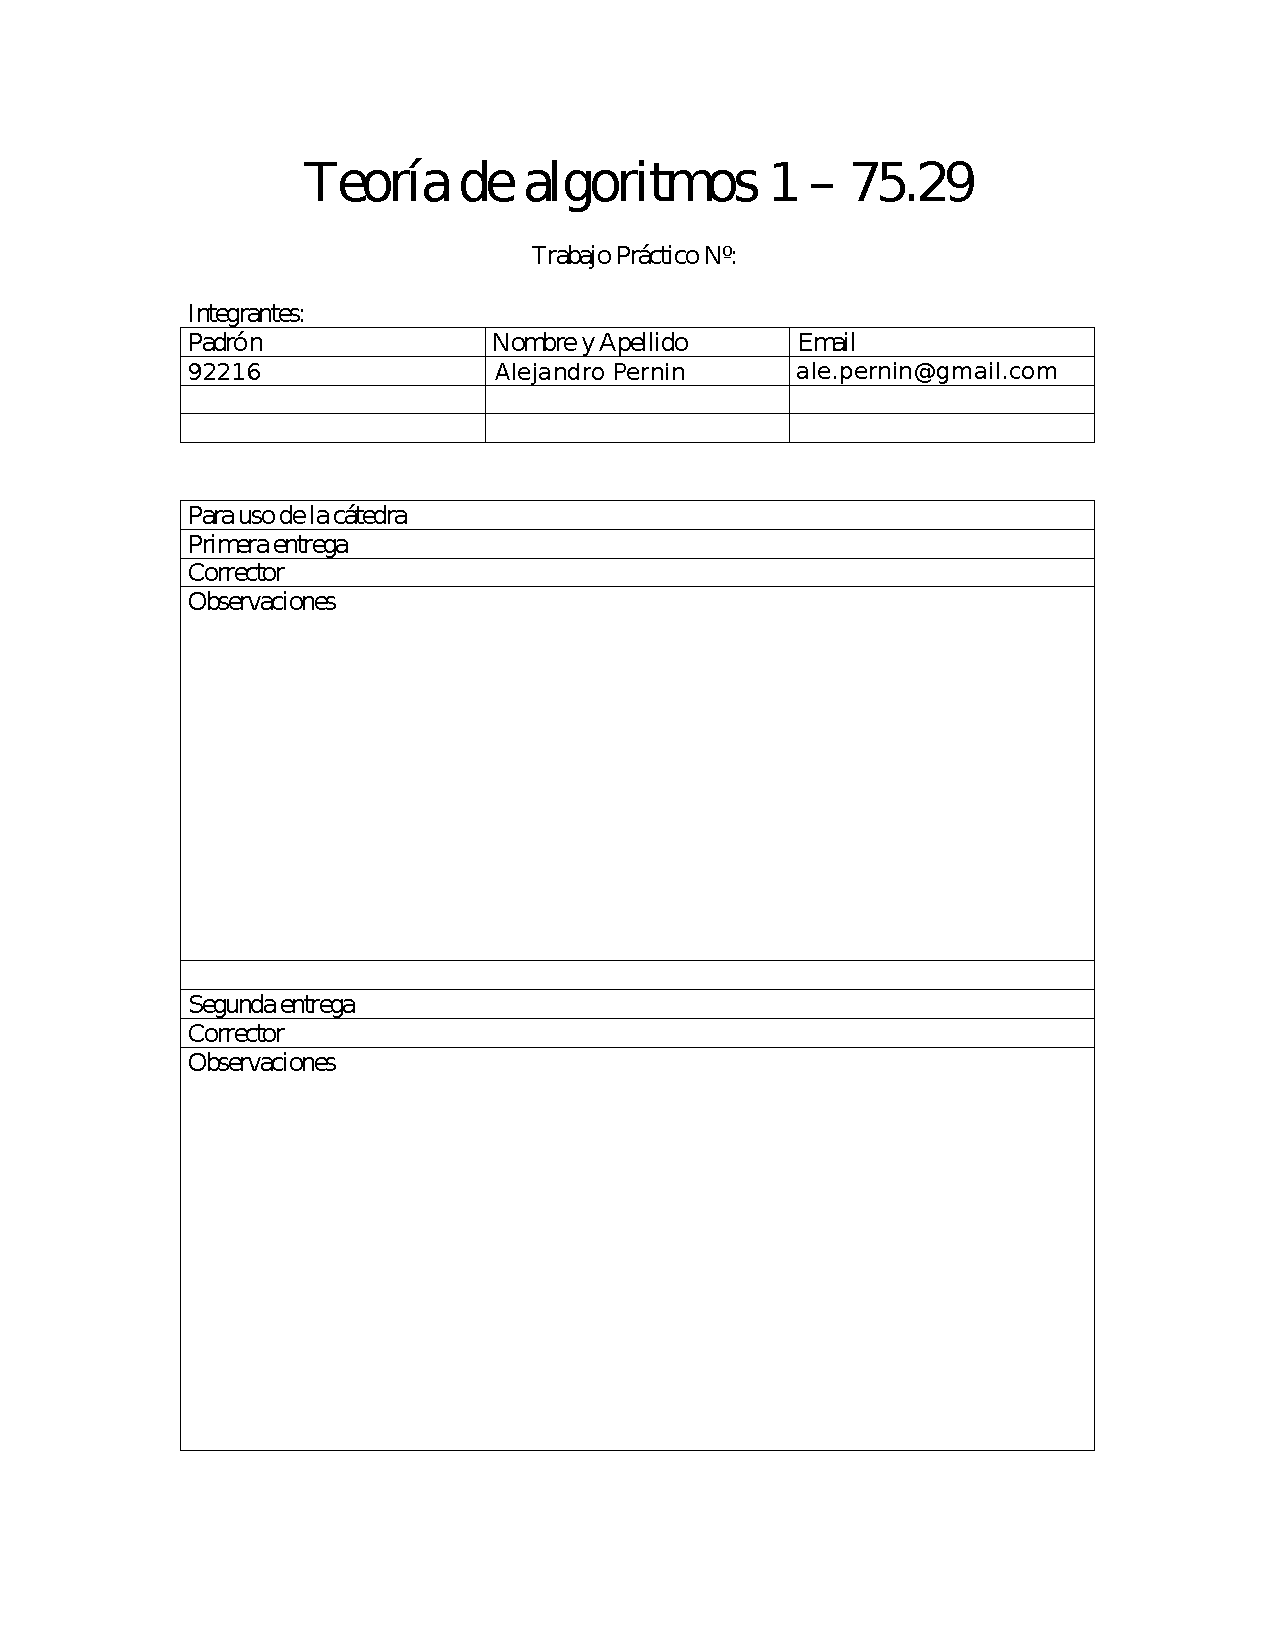
\includepdf{caratulatp.pdf}

\maketitle

\newpage
\tableofcontents

\newpage

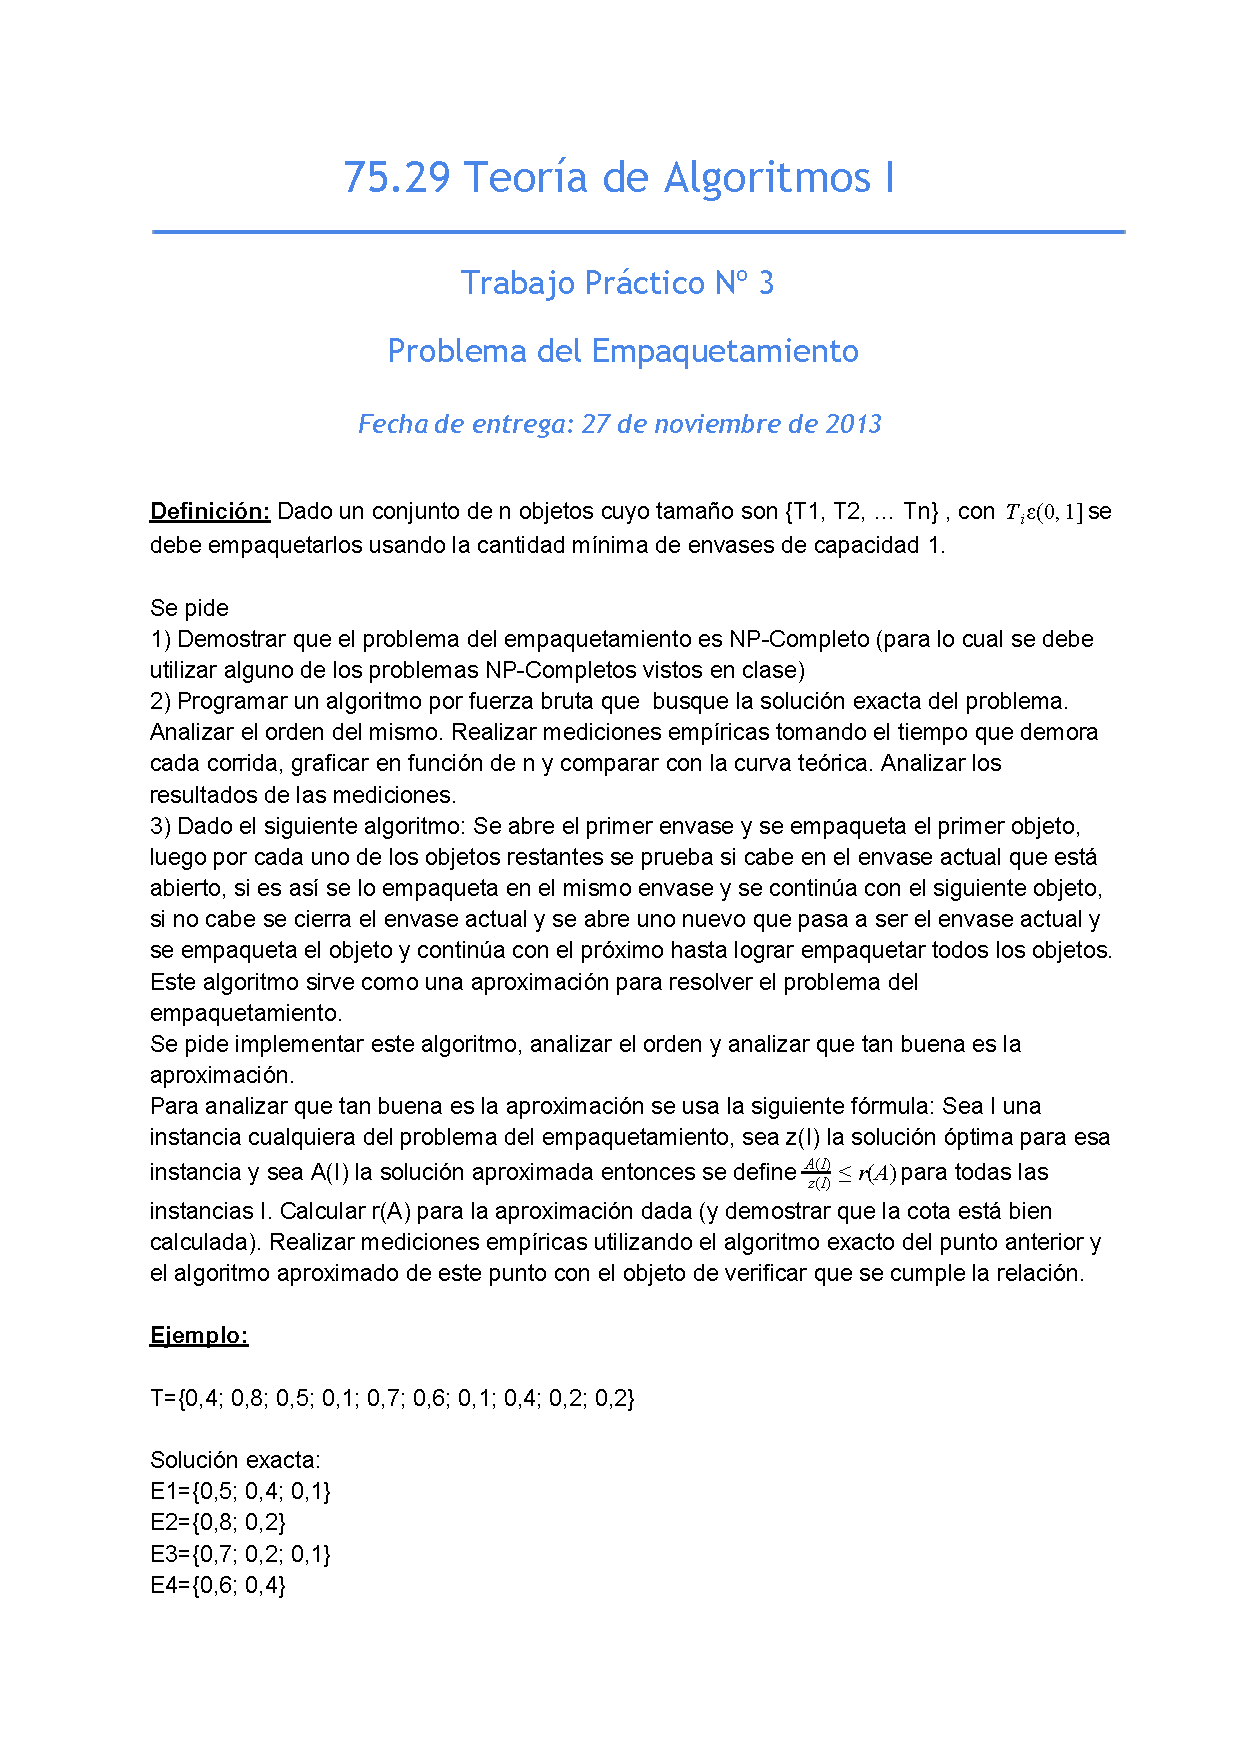
\includepdf[pages=-]{TDATP32013.pdf}

\newpage
\section{Resolucion}
	\subsection{Demostración NP-Completo}
		Para la demostración de que este problema es NP-Completo, se 
		utiliza otro problema cuya demostración de NP-Completo se considera
		ya conocida; reduciendo dicho conocido problema al problema de
		Bin Packing, demostramos que el problema también es NP.
		
		Como problema de referencia se utilizar\'a \emph{Subset Sum}\footnote{\url{http://en.wikipedia.org/wiki/Subset_sum_problem}}.
		Primero definamos ambos problemas como problemas de decisión:
		\begin{itemize}
			\item \underline{Bin Packing}: $\{ <S,j> | S = \{ s_{1},s_{2}...,s_{n}\}; 0<s_{i}<1,$ 
			y todos los objetos $1,...,n$ deben empaquetarse en envases de capacidad $j$.
			
			\item \underline{Subset Sum}: $\{ <C,k> | C = \{ c_{1},c_{2}...,c_{n}\}$ donde $c_{i}$
			es un entero positivo, y existe algun subconjunto $C'\subseteq C$ tal que la suma de sus
			elementos sume exactamente $k$.
		\end{itemize}
		
		Se considera demostrado y sabido que \emph{Subset Sum} es NP-Completo, 
		por medio de reducción demostraremos que \emph{Bin Packing} también lo es.
		Primero consideramos que \emph{Subset Sum} es NP-Completo aún en un caso restringido:
			\\ 
			
			$k=\sum_{c_{i}\in C}^{n} c_{i}/2 = W/2$
			
		Llamamos a esta instancia \emph{Subset Half Sum}, instancia que
		se demostrará se soluciona facilmente con \emph{Bin Packing}. Para
		ello mostramos que una instancia $<C,k>$ de \emph{Subset Half Sum}
		$\leq p$ \emph{Bin Packing} \footnote{Notación ver: Algorithm Desing - Chapter 8, page 452}.
		Primero se convierten los elementos en $C$ a un problema de \emph{Bin Packing}
		de $1$ envase dividiendo los elementos en $C$ por $k$. Eso es, para $C=\{c_{1},c_{2},...,c_{n}\}$
		crear $C'=\{ s_{i} |  s_{i}=c_{i}/k\}$. Creamos una instancia
		$<C',2>$ de \emph{Bin Packing}. Si la respuesta a este \emph{Bin Packing}
		es "si", también lo será para \emph{Subset Half Sum}, de lo contrario "no".
		\\
	
		Prueba: Si el mínimo de envases es 2 y cada envase tiene capacidad $\frac{W}{2k}$,
		 entonces cada uno contiene un subconjunto de peso esactamente $\frac{W}{2k}$, y
		 cada uno es una solución a \emph{Subset Half Sum}. Si el mínimo de envases
		 es mayor a 2(no puede ser 1 ya que $1<W/k$), no existe ningún subconjunto de peso $\frac{W}{2k}$. De 
		 otro modo, tendriamos que usar ese subconjunto en el primer envase y los
		 $\frac{W}{2}$ items en el segundo envase obteniendo una solución de 2 envases.
	
	\subsection{Fuerza Bruta}
		La resolución por fuerza bruta, implica probar todas las combinaciones 
		posibles y de ellas obtener la que implique el menor uso de envases.
		El enfoque que se utiliza en este TP, es por cada combinación posible
		con los elementos del cojunto, correr el algoritmo de aproximación, 
		bajo la hipótesis de que existe al menos una permutación del conjunto
		para el cuál el algoritmo de aproximación da el resultado óptimo.
		
		Para hacer un análisis del mismo es preciso primero analizar cuantas
		permutaciones posibles hay a partir de un conjunto, para ello
		se analiza desde un punto de vista recurrente. Sea el conjunto 
		$S=\{s_{1},s_{2},...,s_{n}\}$ y la función $P(n)$ que dá la cantidad
		de permutaciones para un conjunto de $n$ elementos, $P(n)=n*P(n-1)$.
		El caso base sería $P(1)=1$ lo cuál es trivial ya que no hay permutaciones
		posibles para un elemento más que él mismo. Armando el arbol de 
		recurrencias se llega a que $P(n)=n!$
	
		Con motivo de analizar los tiempos que demanda la ejecución del programa,
		se toma el tiempo en el cuál se inició y concluyó, siendo la resta
		de los mismos el tiempo que tardó. El mismo se expresa en milisegundos y
		los valores cercanos a 0 son propensos a mayores errores relativos.
		
		Para las pruebas se efectuaron datos al azar y ejecutaron varias veces,
		siendo el tiempo que se mostrará el promedio de los tiempos obtenidos.
		Para las pruebas de conjuntos de tamaños considerables (10 y 11) solo
		se efectuo una ejecución por el tiempo que llevaría hacer varias
		ejecuciones.
		
			\begin{center}
		 \begin{tabular}{|l|l|l|} \hline
		 	n &$fact(n)$ & tiempo ms \\ \hline
			1 & 1 & 0.068 \\ \hline
			2 & 2 & 0.078 \\ \hline
			3 & 6 & 0.11\\ \hline
			4 & 24 &  0.5\\ \hline
			5 & 120 &  2.57\\ \hline
			6 & 720 &  14.16\\ \hline
			7 & 5040 &  92.3\\ \hline
			8 & 40320 & 716.91\\ \hline
			9 & 362880 &  7238.83\\ \hline
			10 & 3628800&  78387\\ \hline
			11 & 39916800 & 1138704 \\ \hline
		\end{tabular}
		
		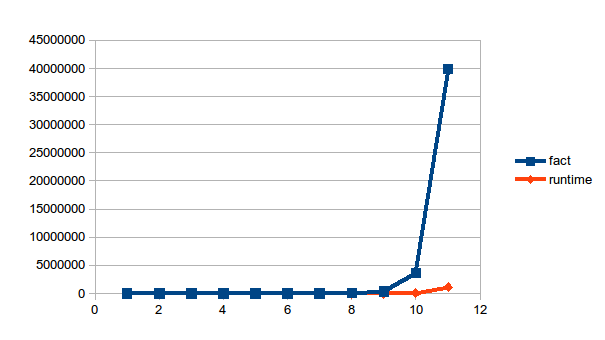
\includegraphics{graf.png}
	\end{center} 
		Aunque en el gráfico no se aprecie con exactitud, en la tabla es
		apreciable como los tiempos crecen factorialmente
\newpage
\section{Analisis de Orden}\label{sec:orden}		
		
\newpage
\section{Codigo Fuente}\label{sec:cf}
\end{document}
